\documentclass[10pt,pdf,hyperref={unicode}]{beamer}


%\documentclass[10pt]{beamer}

\usetheme[progressbar=frametitle]{metropolis}

\usepackage{booktabs}
\usepackage[scale=2]{ccicons}

\usepackage{pgfplots}

\usepgfplotslibrary{dateplot}

\usepackage{xspace}
\newcommand{\themename}{\textbf{\textsc{metropolis}}\xspace}

\usepackage{multicol}
%\usepackage{lmodern}

% подключаем кириллицу 
\usepackage[T2A]{fontenc}
\usepackage[utf8]{inputenc}
\usepackage{listings}
%\usepackage{graphicx}
\usepackage{hyperref}

% отключить клавиши навигации
\setbeamertemplate{navigation symbols}{}

% тема оформления
\usetheme{Pittsburgh}

% цветовая схема
\usecolortheme{default}

\definecolor{light-gray}{gray}{0.90}

\title{Семинар №8}   
\subtitle{ФАКТ \the\year}
\author{Бирюков В. А.} 
\date{\today}
% \logo{
\includegraphics[height=5mm]{images/logo.png}\vspace{-7pt}}

\begin{document}

\lstset{language=C}

% титульный слайд
\begin{frame}
\titlepage
\end{frame} 

\lstset{
  language=C,                % choose the language of the code
  basicstyle=\linespread{1.1}\ttfamily,
  columns=fixed,
  fontadjust=true,
  basewidth=0.5em,
  keywordstyle=\color{blue}\bfseries,
  commentstyle=\color{gray},
  stringstyle=\ttfamily\color{orange!50!black},
  showstringspaces=false,
  numbersep=5pt,
  numberstyle=\tiny\color{black},
  numberfirstline=true,
  stepnumber=1,                   % the step between two line-numbers.        
  numbersep=10pt,                  % how far the line-numbers are from the code
  backgroundcolor=\color{black!2},  % choose the background color. You must add \usepackage{color}
  showstringspaces=false,         % underline spaces within strings
  captionpos=b,                   % sets the caption-position to bottom
  breaklines=true,                % sets automatic line breaking
  breakatwhitespace=true,         % sets if automatic breaks should only happen at whitespace
  xleftmargin=.2in,
  extendedchars=\true,
  keepspaces = true,
}
\lstset{literate=%
   *{0}{{{\color{red!20!violet}0}}}1
    {1}{{{\color{red!20!violet}1}}}1
    {2}{{{\color{red!20!violet}2}}}1
    {3}{{{\color{red!20!violet}3}}}1
    {4}{{{\color{red!20!violet}4}}}1
    {5}{{{\color{red!20!violet}5}}}1
    {6}{{{\color{red!20!violet}6}}}1
    {7}{{{\color{red!20!violet}7}}}1
    {8}{{{\color{red!20!violet}8}}}1
    {9}{{{\color{red!20!violet}9}}}1
}


\section{Хранение переменных и массивов в памяти}
\begin{frame}[fragile]
\frametitle{Шестнадцатеричная система} 
Система счисления по целочисленному основанию \texttt{16}. \\ 
В качестве цифр этой системы обычно используются цифры от \texttt{0} до \texttt{9} и латинские буквы от \texttt{A} до \texttt{F}.\\
Примеры:\\
\begin{multicols}{2}
\texttt{6 = 0x6} \\
\texttt{12 = 0xc} \\
\texttt{20 = 0x14} \\
\texttt{200 = 0xc8} \\
\texttt{255 = 0xff} \\
\texttt{256 = 0x100} \\
\texttt{1000 = 0x3E8} \\
\texttt{1024 = 0x400} \\
\end{multicols}
\end{frame}

\begin{frame}[fragile]
\frametitle{Шестнадцатеричная система} 
Пример работы шестнадцатиричной системой в языке C:\\
Вместо \texttt{\%d} (decimal) используем \texttt{\%x} (hexadecimal)
\begin{lstlisting}
#include <stdio.h>
int main()
{
	int a = 1000;
	printf("%d\n", a);
	printf("%x\n", a);
}
\end{lstlisting}
\end{frame}

\begin{frame}[fragile]
\frametitle{Шестнадцатеричная система} 
Для создания шестнадцатиричного числа нужно дописать 
к числу приставку \texttt{0x}
\begin{lstlisting}
#include <stdio.h>
int main()
{
	int a = 0x14;
	printf("%d\n", a);
	printf("%x\n", a);
}
\end{lstlisting}
\end{frame}

\begin{frame}[fragile]
\frametitle{Хранение переменных типа \texttt{int} в памяти}
Предположим, что мы создали переменную типа \texttt{int} в памяти и присвоили ей число \texttt{7570004}.\\
Как это число будет выглядеть в памяти?\\
Если это число перевести в 16-ричную систему, то получится \texttt{0x738254}.
\begin{center}
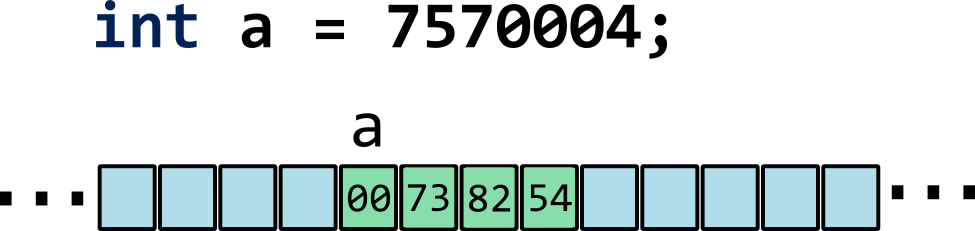
\includegraphics[width=0.72\linewidth]{../images/memory/memory_0_int_dec.png}
\end{center}
\end{frame}

\begin{frame}[fragile]
\frametitle{Хранение переменных типа \texttt{int} в памяти} 
\begin{center}
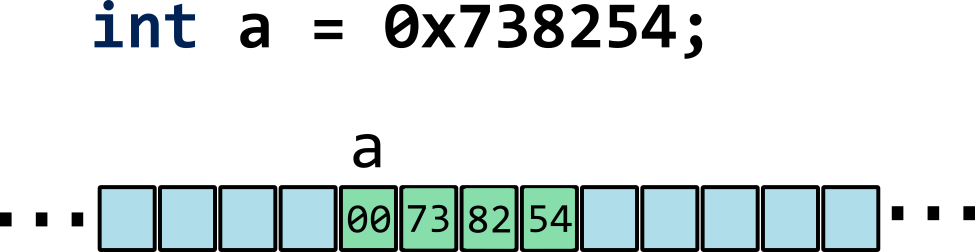
\includegraphics[width=0.72\linewidth]{../images/memory/memory_0_int_hex.png}
\end{center}
\end{frame}

\begin{frame}[fragile]
\frametitle{Порядок байт}
Порядок байт:
\begin{enumerate}
\item Big Endian -- от старшего байта к младшему.
\item Little Endian  -- от младшего байта к старшему. Используется в большинстве вычислительных системах.
\end{enumerate}
\begin{center}
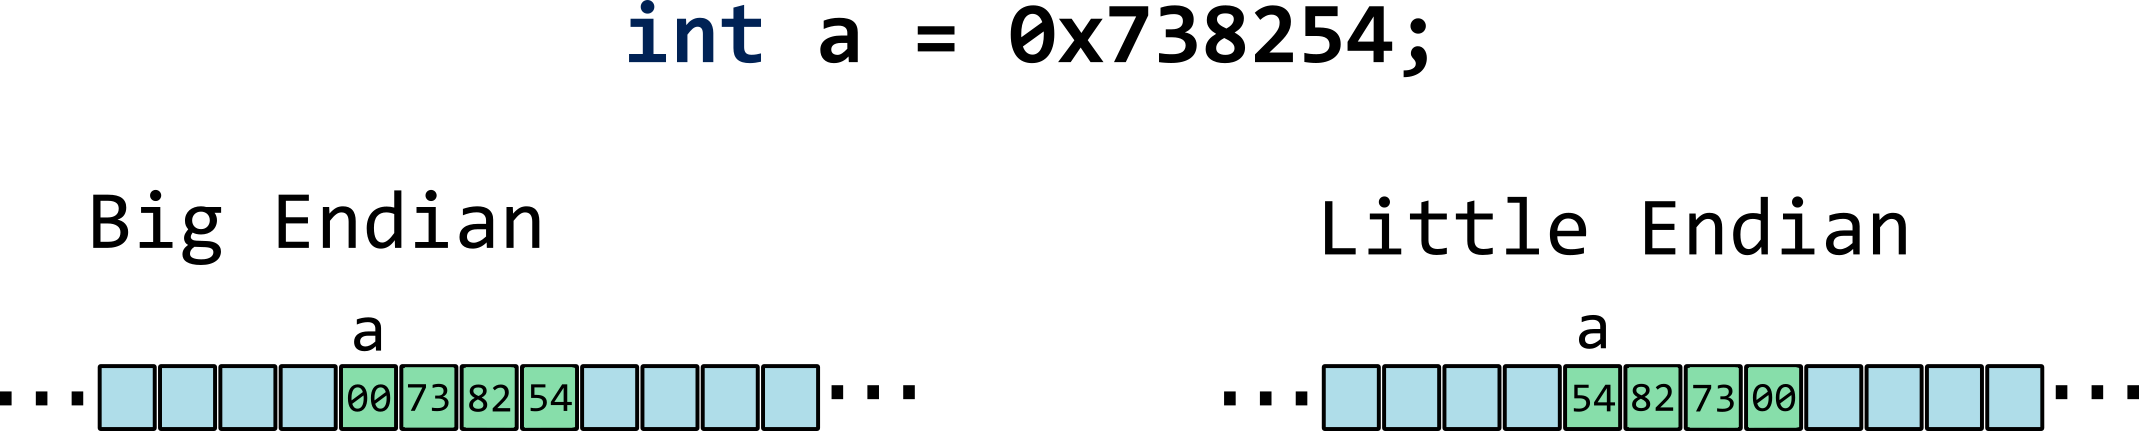
\includegraphics[width=0.86\linewidth]{../images/memory/memory_1_endianness.png}
\end{center}
В дальнейшем будем предполагать, что используется порядок Little Endian
\end{frame}

\begin{frame}[fragile]
\frametitle{Разные переменные в памяти} 
\begin{center}
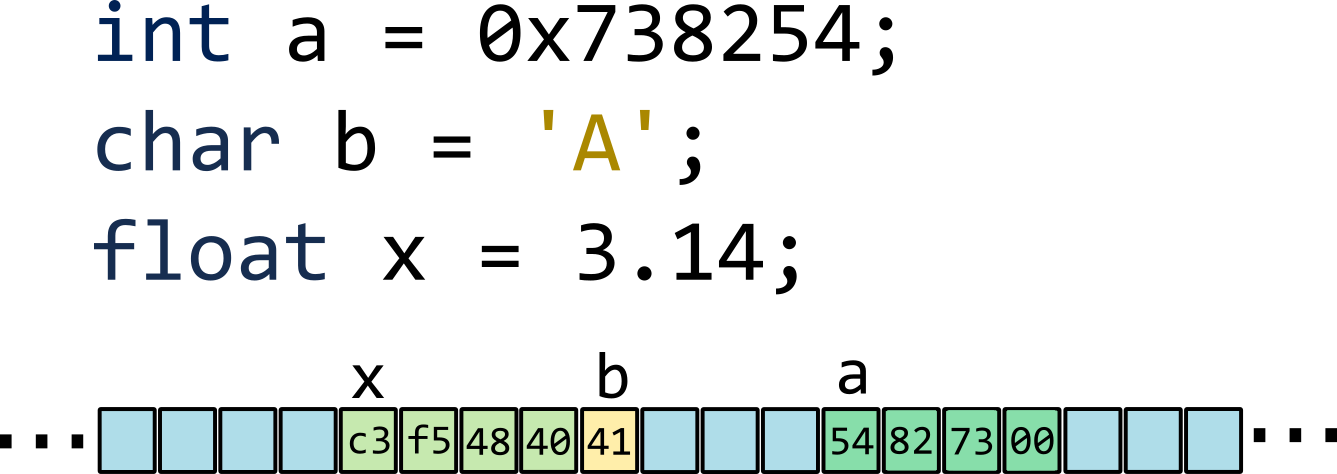
\includegraphics[width=0.86\linewidth]{../images/memory/memory_2_different_types.png}
\end{center}
\end{frame}

\begin{frame}[fragile]
\frametitle{Указатель на переменную типа \texttt{int}}
Каждый ячейка памяти имеет номер (адрес).\\
Указатель -- переменная, которая хранит адреса.
\begin{center}
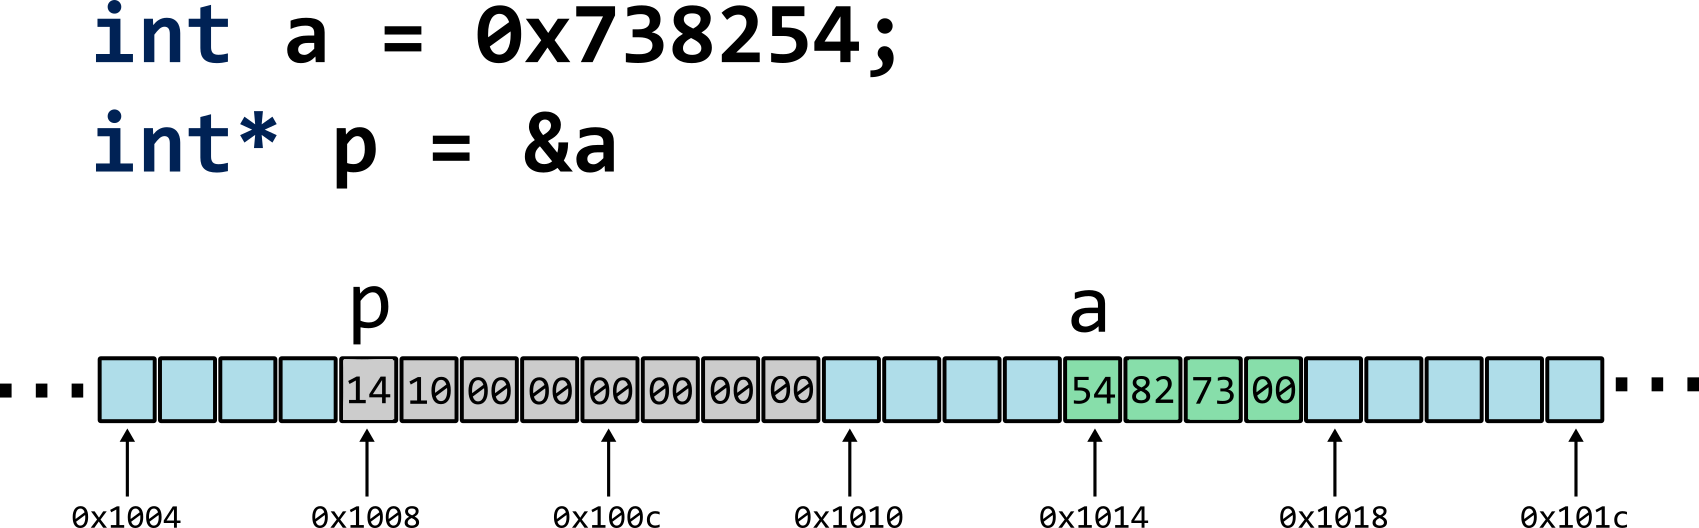
\includegraphics[width=0.86\linewidth]{../images/memory/memory_3_pointer_to_int.png}
\end{center}
В 64-х битных система размер указателя равен 64 бит \\(т.е. 8 байт).\\
Обратите внимание, что для указателя тоже используется Little Endian.
\end{frame}

\begin{frame}[fragile]
\frametitle{Указатель на переменную типа \texttt{char}} 
\begin{center}
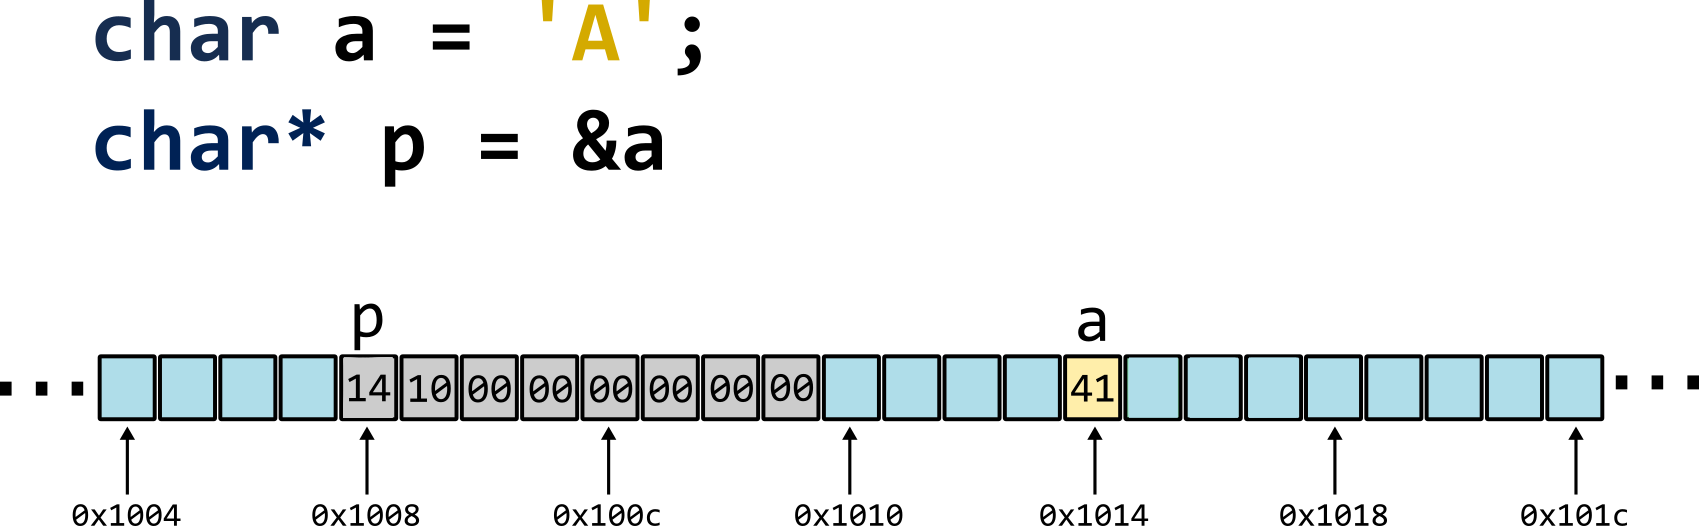
\includegraphics[width=0.86\linewidth]{../images/memory/memory_4_pointer_to_char.png}
\end{center}
Код ASCII символа A равен 65 или 0x41. \\
Независимо от размера самой переменной, размер указателя равен 8 байтам.
\end{frame}

\begin{frame}[fragile]
\frametitle{Указатель на переменную типа \texttt{double}} 
\begin{center}
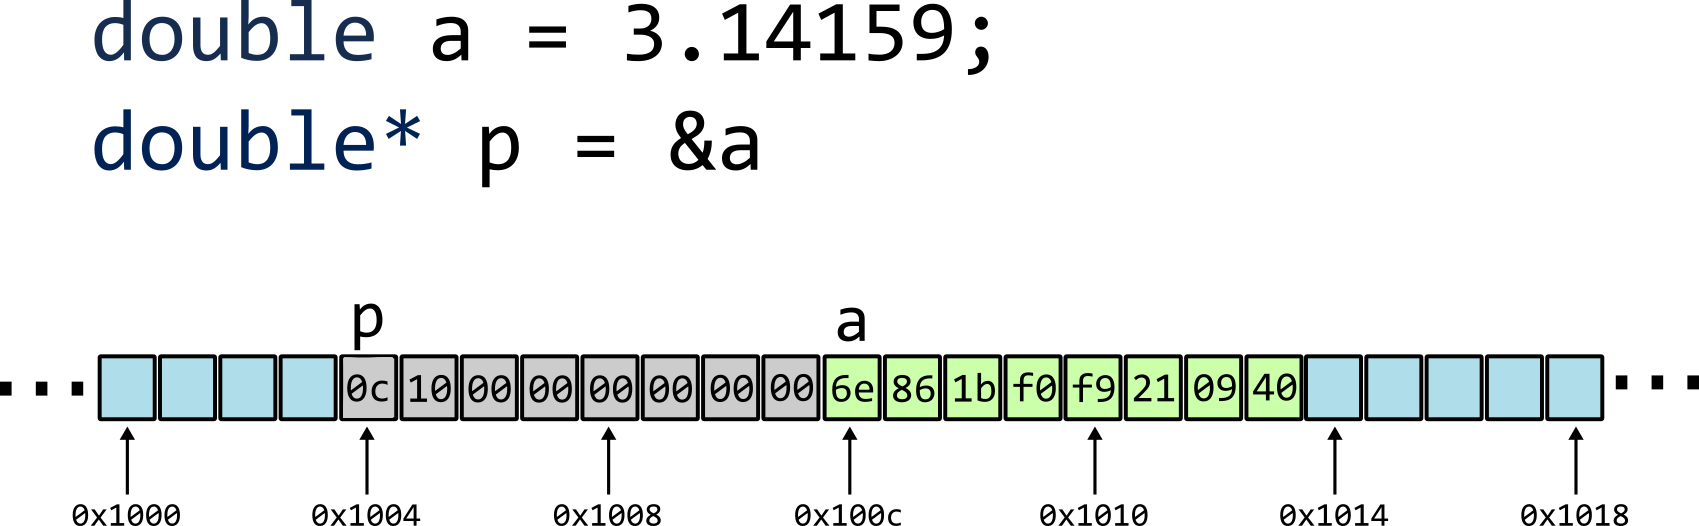
\includegraphics[width=0.86\linewidth]{../images/memory/memory_5_pointer_to_double.png}
\end{center}
Представление чисел с плавающей точкой в памяти задаётся стандартом \texttt{IEEE 754}.\\
Шестнадцатиричное представление \texttt{3.14159} по этому стандарту: \texttt{0x400921f9f01b866e}.
\end{frame}

\begin{frame}[fragile]
\frametitle{Указатель на элемент массива \texttt{int}-ов} 
Элементы массива лежат в памяти последовательно, без зазоров. 
Порядок байт -- обратный, но только в рамках одного базового типа.
\begin{center}
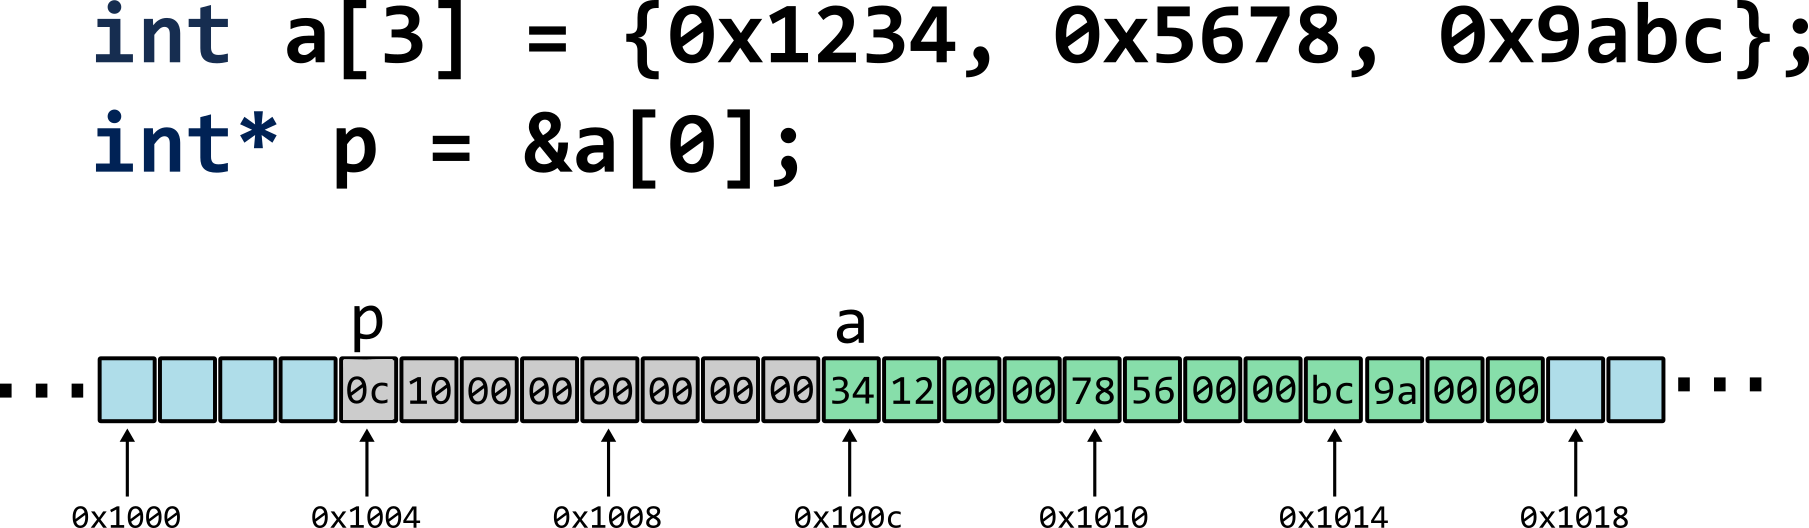
\includegraphics[width=0.86\linewidth]{../images/memory/memory_6_pointer_to_int_array.png}
\end{center}
\end{frame}

\begin{frame}[fragile]
\frametitle{Указатель на элемент массива \texttt{int}-ов} 
При присваивание указателю или при передаче в функцию 
название массива ведёт себя как указатель на первый 
элемент (т. е. \texttt{a == \&a[0]})
\begin{center}
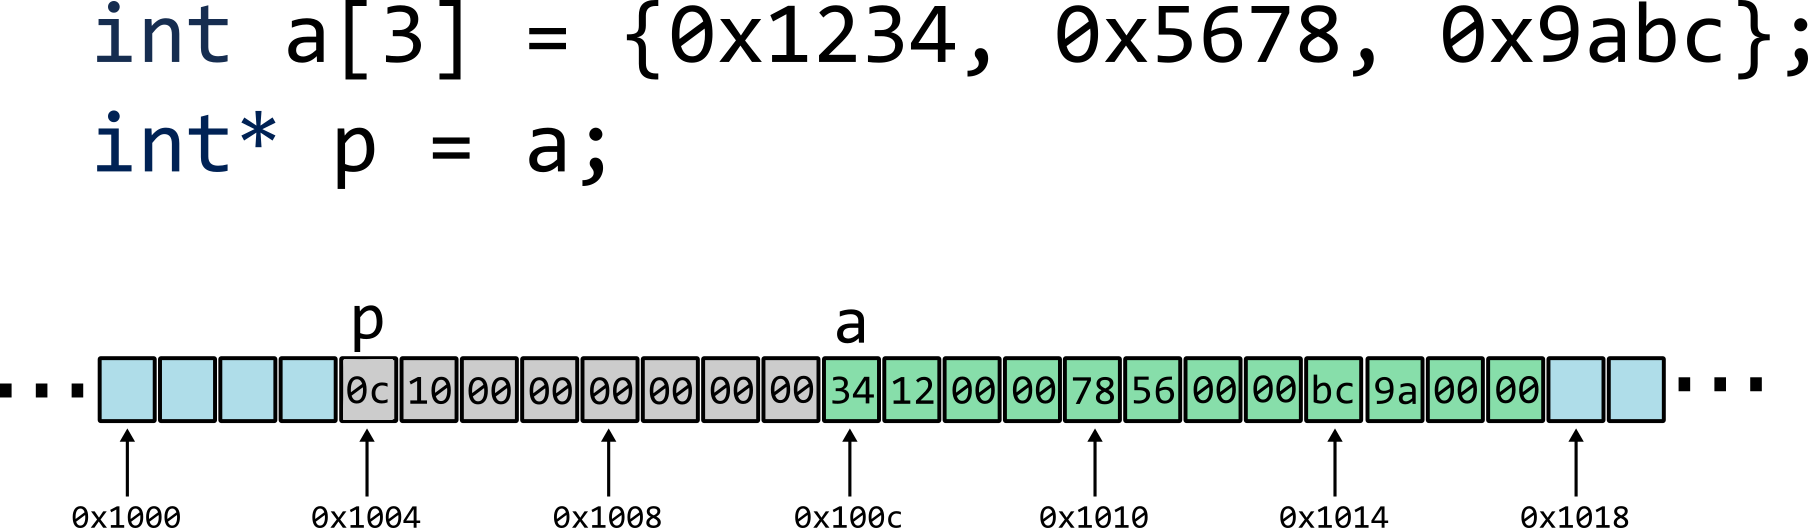
\includegraphics[width=0.86\linewidth]{../images/memory/memory_6_pointer_to_int_array_by_name.png}
\end{center}
\end{frame}

\begin{frame}[fragile]
\frametitle{Указатель на элемент массива \texttt{char}-ов (строку)} 
Символ \texttt{M} имеет код ASCII равный \texttt{77 = 0x4d}.\\
Остальные символы:\\
\texttt{I} (\texttt{0x49}), \texttt{P} \texttt{(0x50}), \texttt{T}(\texttt{0x54}) \texttt{!}(\texttt{0x21})
\begin{center}
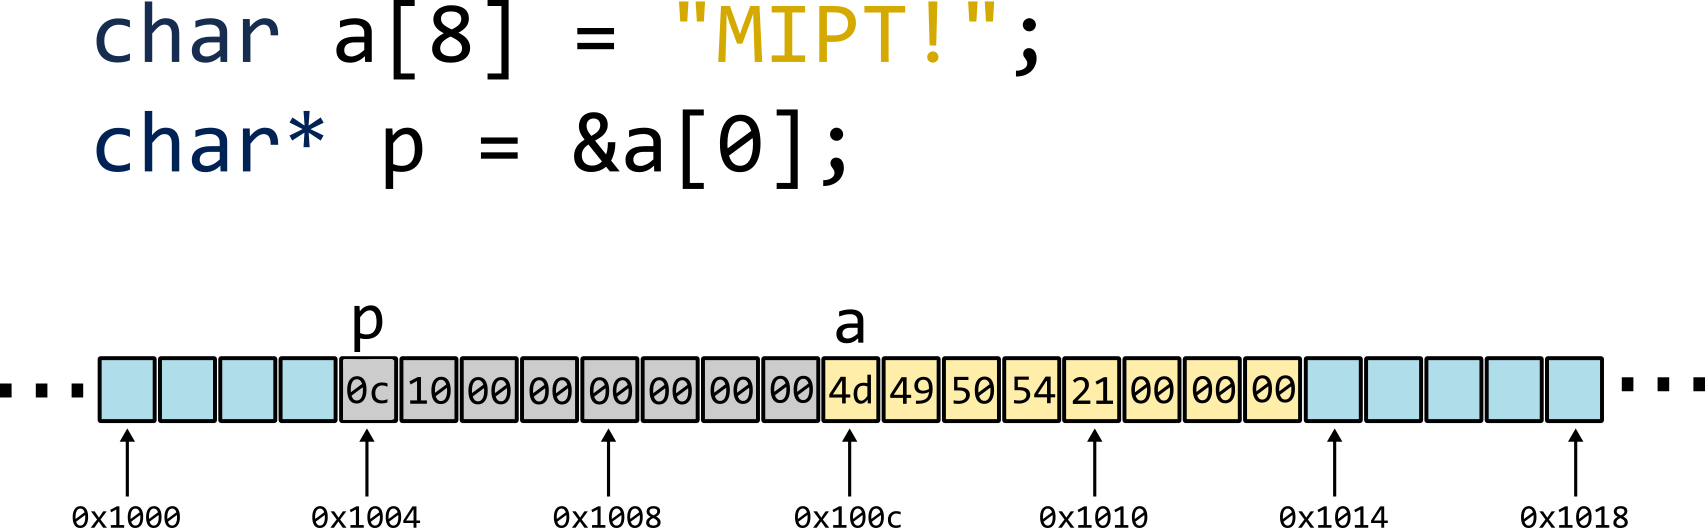
\includegraphics[width=0.86\linewidth]{../images/memory/memory_7_pointer_to_char_array.png}
\end{center}
\end{frame}


\begin{frame}[fragile]
\frametitle{Схематическое изображение указателя} 
Так как постоянно рисовать память и адреса затратно,
то будем использовать схематическое изображение обычных переменных (в виде прямоугольника)
 и указателей (в виде прямоугольничка со стрелочкой)
\begin{center}
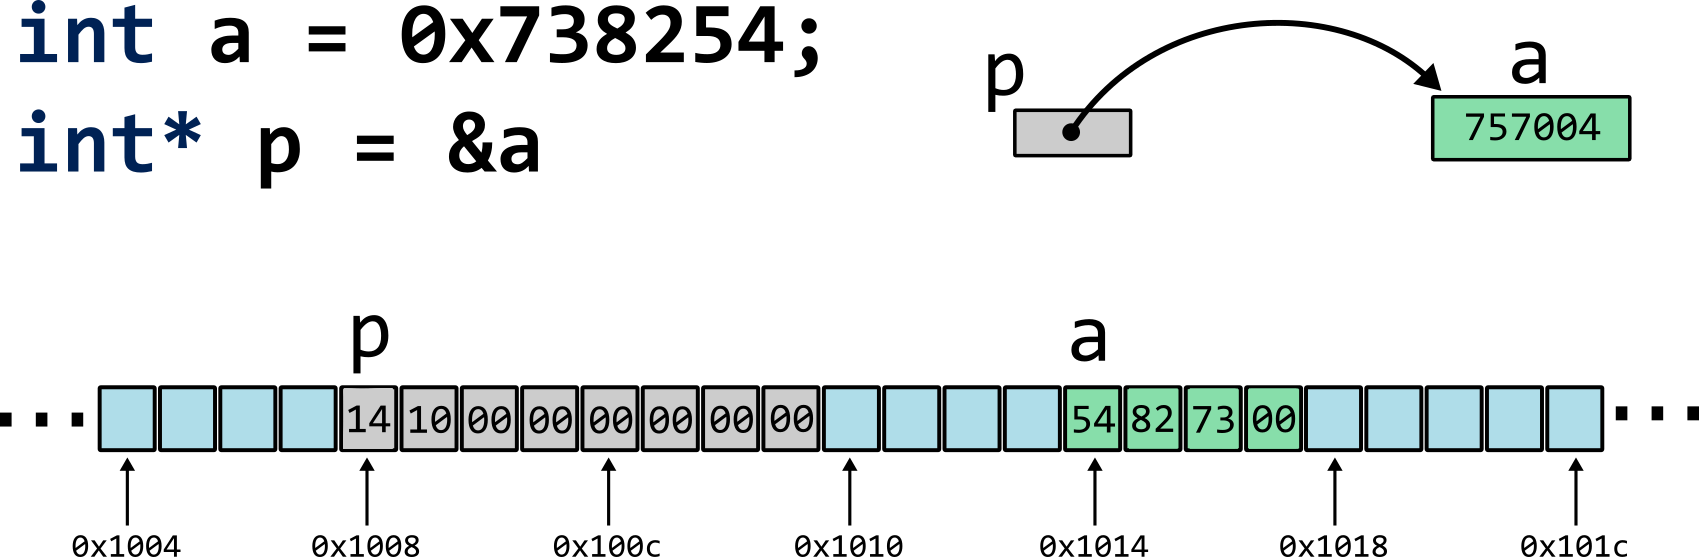
\includegraphics[width=0.86\linewidth]{../images/memory/memory_8_schematic.png}
\end{center}
\end{frame}

\begin{frame}[fragile]
\frametitle{Схематическое изображение указателя на элемент массива} 
\begin{center}
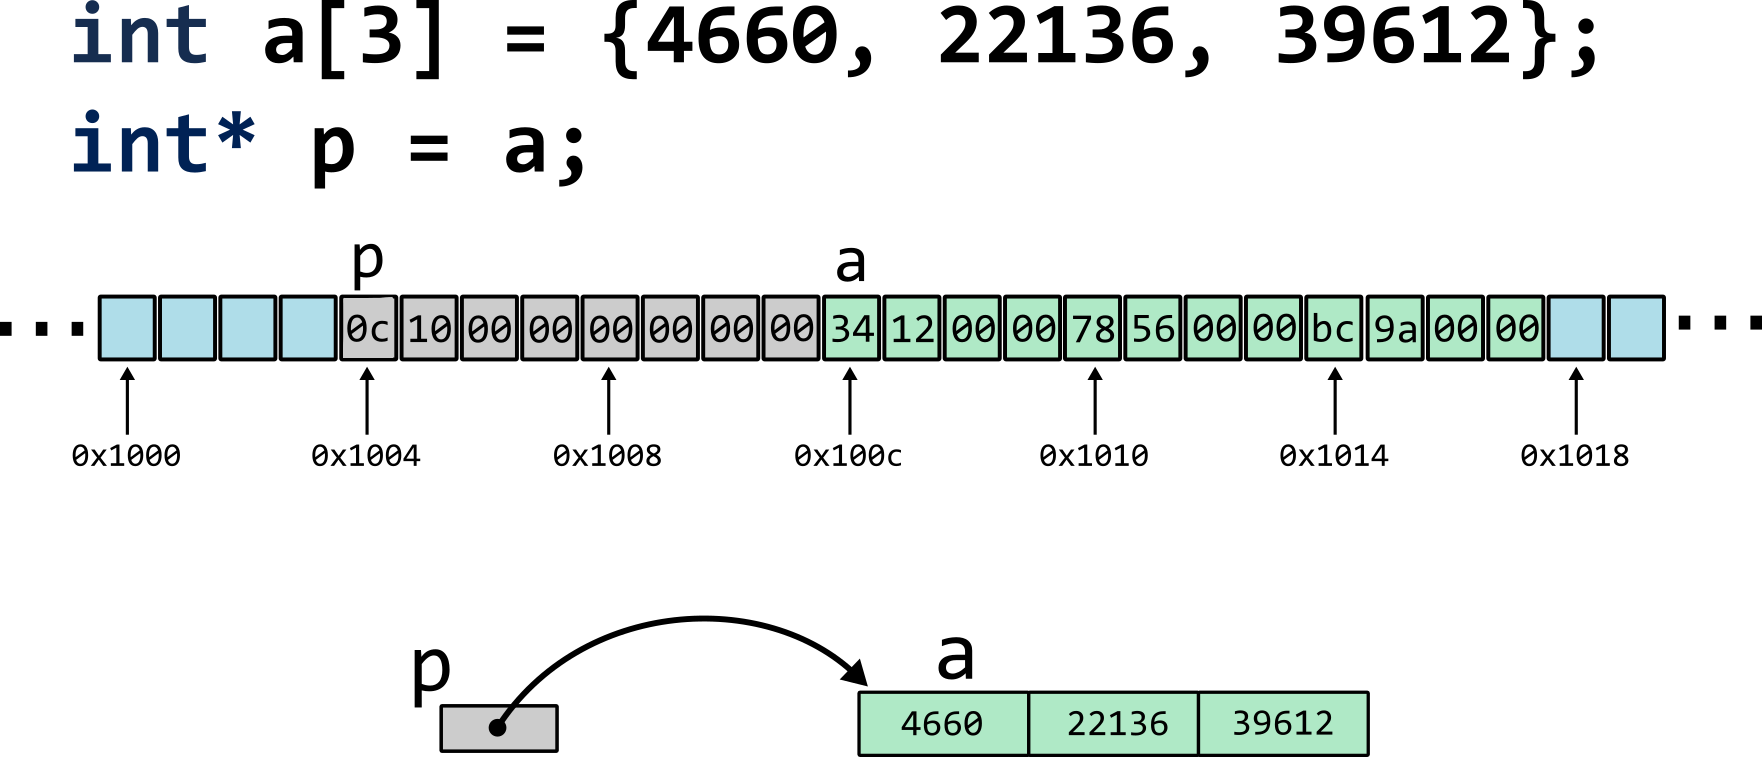
\includegraphics[width=0.86\linewidth]{../images/memory/memory_9_schematic_int_array.png}
\end{center}
Так как \texttt{4660 = 0x1234}, \texttt{22136 = 0x5678} и \\ \texttt{39612 = 0x9abc}.
\end{frame}


\section{Арифметика указателей}

\begin{frame}[fragile]
\frametitle{Операции с указателями}
\begin{lstlisting}
int array[5] = {11, 12, 13, 14, 15};
int* p = &array[0];
int* q = &array[3];
\end{lstlisting}
\begin{itemize}
\item Прибавление/вычитание целого числа
\begin{verbatim}
p += 2;
\end{verbatim}
\item Вычитание двух указателей
\begin{verbatim}
int n = q - p;
\end{verbatim}
\item Разыменование
\begin{verbatim}
int x = *p;
\end{verbatim}
\item Квадратные скобки
\begin{verbatim}
int x = p[2];
\end{verbatim}
\end{itemize}
\end{frame}


\begin{frame}[fragile]
\frametitle{Указатель на массив \texttt{int}-ов} 
\begin{center}
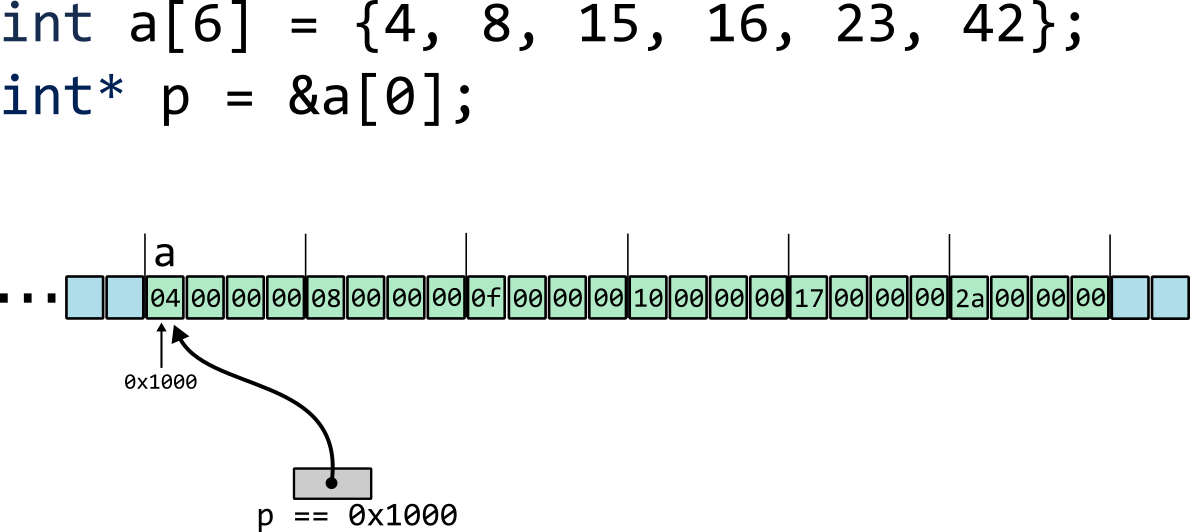
\includegraphics[width=0.86\linewidth]{../images/pointer_arithmetics/parithmetics_0_initial_int.png}
\end{center}
\end{frame}

\begin{frame}[fragile]
\frametitle{Указатель на массив \texttt{int}-ов} 
\begin{center}
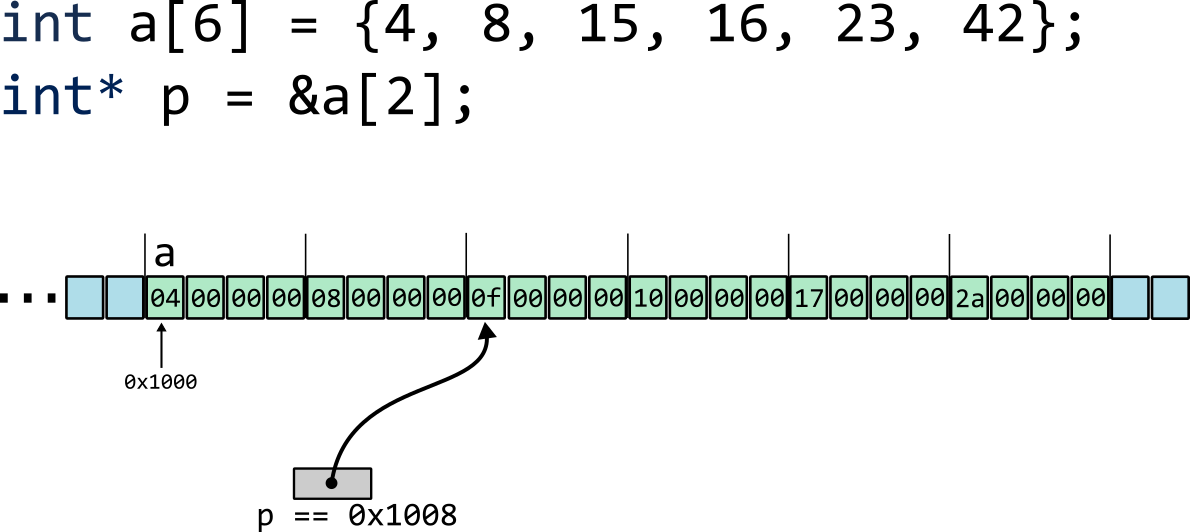
\includegraphics[width=0.86\linewidth]{../images/pointer_arithmetics/parithmetics_1_initial_int.png}
\end{center}
\end{frame}

\begin{frame}[fragile]
\frametitle{Прибавление целого числа} 
При прибавлении целого числа \texttt{x} к указателю типа \texttt{int*}, 
указатель увеличивается на \texttt{x * sizeof(int)}
\begin{center}
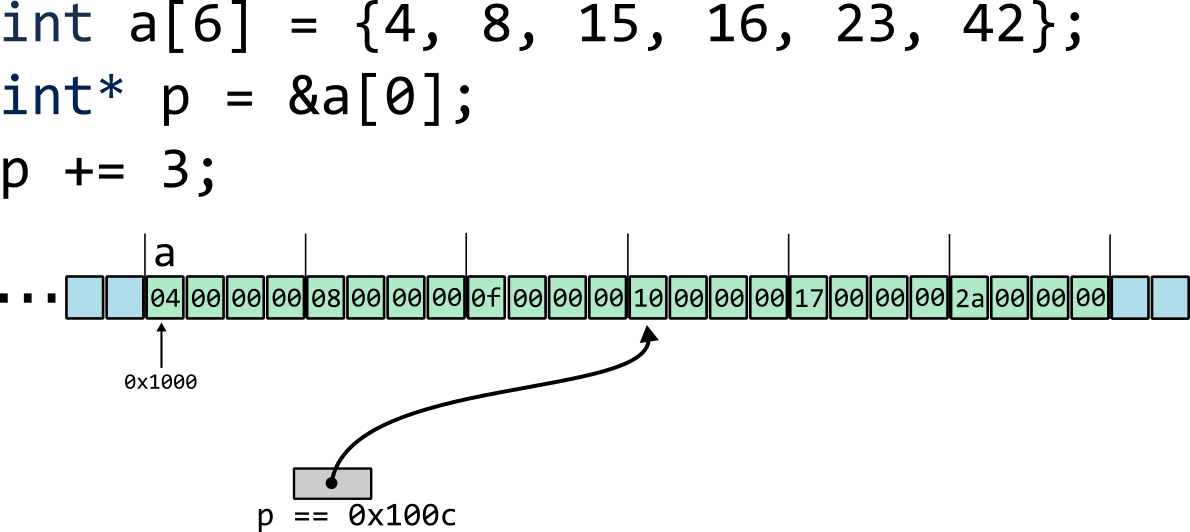
\includegraphics[width=0.86\linewidth]{../images/pointer_arithmetics/parithmetics_2_addition.png}
\end{center}
При прибавлении к \texttt{p} числа 3, указатель увеличился на \texttt{12}.
\end{frame}

\begin{frame}[fragile]
\frametitle{Вычитание целого числа} 
\begin{center}
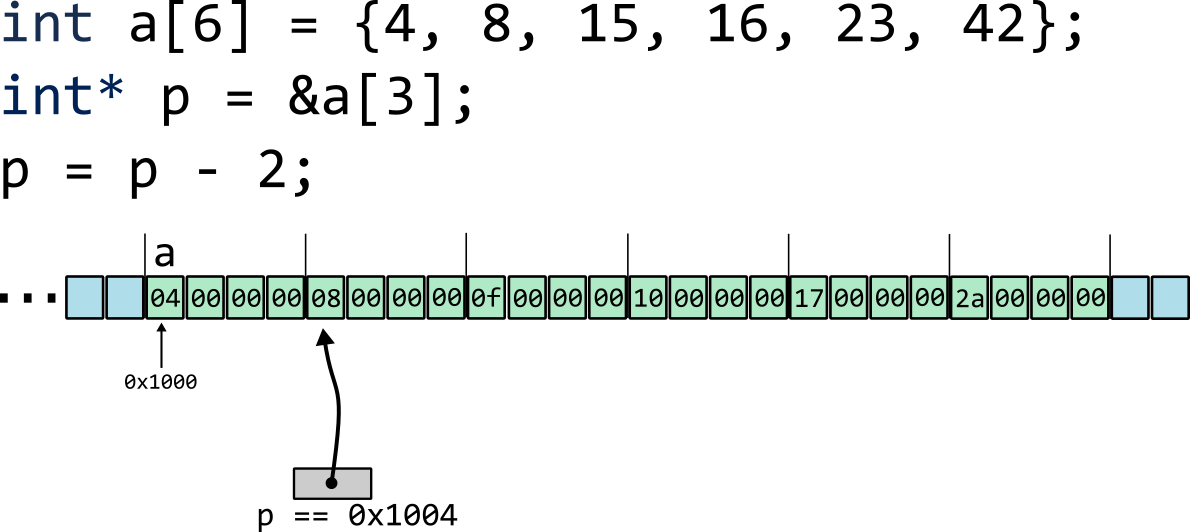
\includegraphics[width=0.95\linewidth]{../images/pointer_arithmetics/parithmetics_3_subtraction.png}
\end{center}
\end{frame}

\begin{frame}[fragile]
\frametitle{Вычитание указателей} 
При вычитании указателей, результат делится на размер типа на который они указывают.
\begin{center}
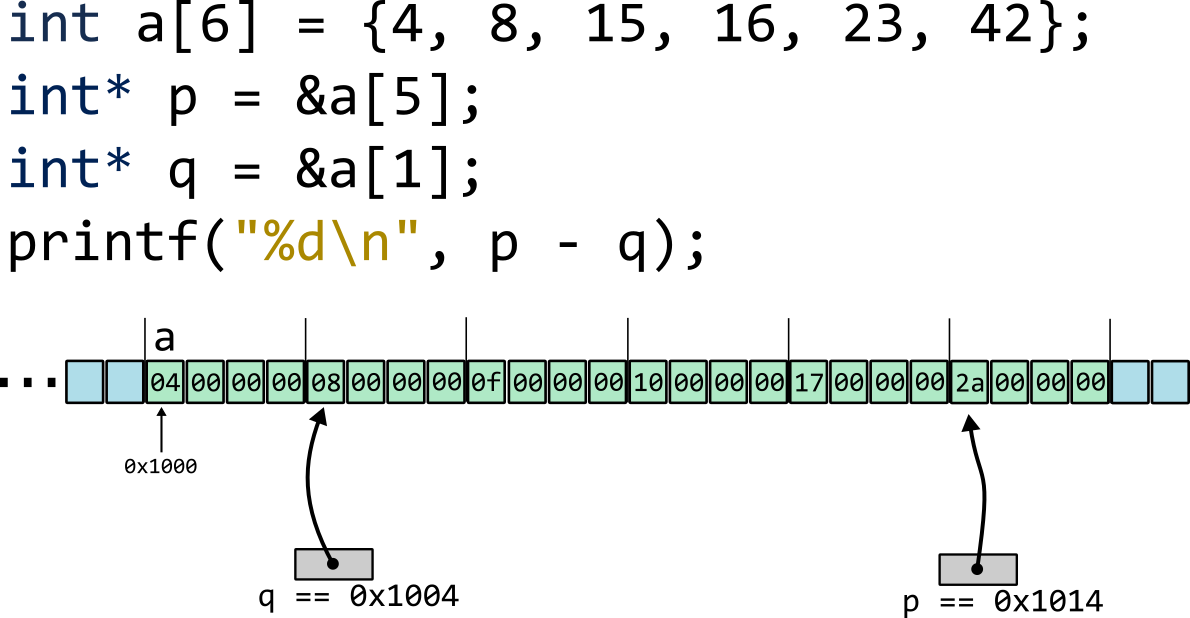
\includegraphics[width=0.86\linewidth]{../images/pointer_arithmetics/parithmetics_4_pointer_subtraction.png}
\end{center}
\texttt{0x1014 - 0x1004 = 0x10 = 16}, но \texttt{p - q = 4}.
\end{frame}


\begin{frame}[fragile]
\frametitle{Разыменование указателя}
Разыменование означает -- пойди по адресу \texttt{p} и воспринимай 4 байта по этому адресу как
переменную типа \texttt{int}
\begin{center}
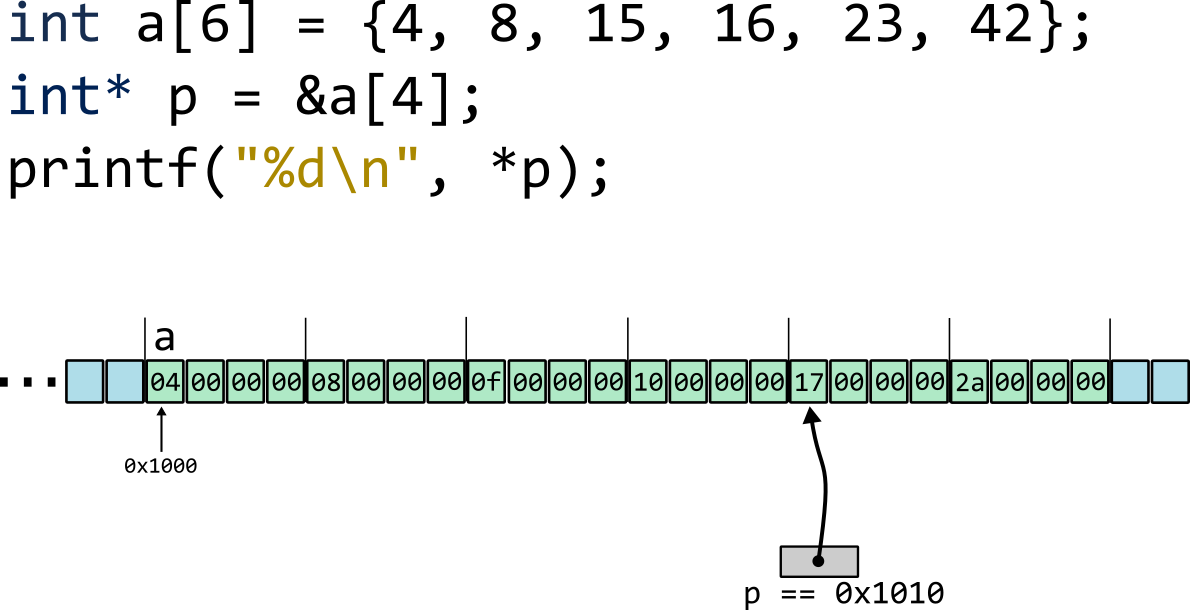
\includegraphics[width=0.86\linewidth]{../images/pointer_arithmetics/parithmetics_5_dereferencing.png}
\end{center}
\end{frame}

\begin{frame}[fragile]
\frametitle{Скобочки}
Скобочки заменяются на разыменование: 
\begin{center}
\texttt{p[i] = *(p + i)}
\end{center}
\begin{center}
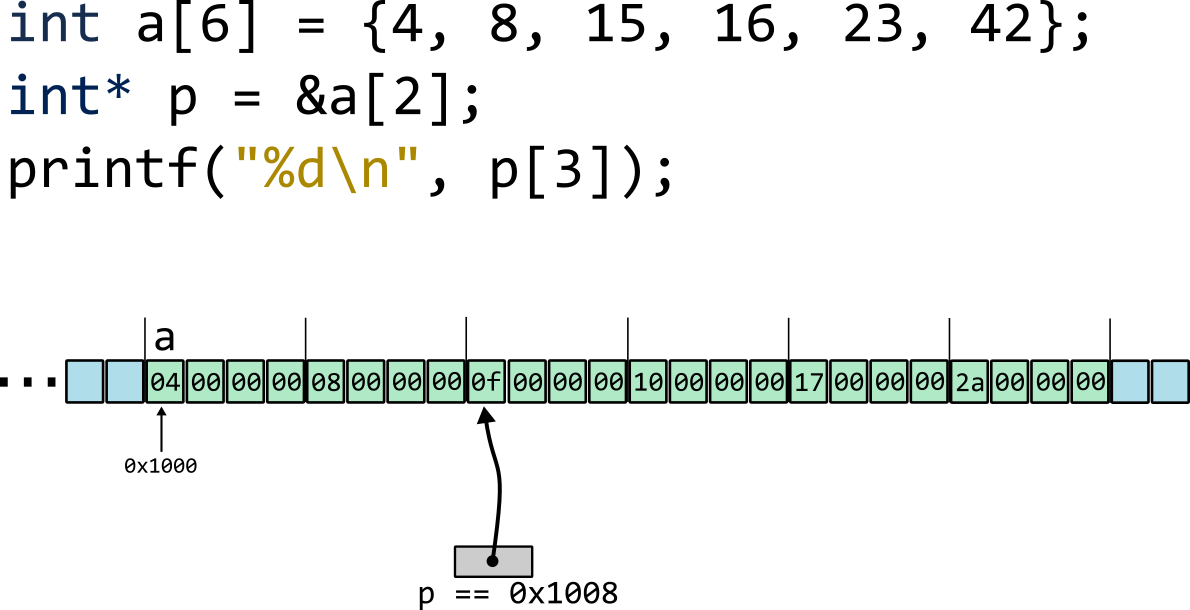
\includegraphics[width=0.86\linewidth]{../images/pointer_arithmetics/parithmetics_6_brackets.png}
\end{center}
\end{frame}

\begin{frame}[fragile]
\frametitle{Приведение указателей} 
\begin{itemize}
\item Приведение типов int и float: \\
\begin{lstlisting}[language=C++,basicstyle=\ttfamily,keywordstyle=\color{blue}]
float x = 5.2;
int y = (int)x;       // явное
int z = x;            // неявное
\end{lstlisting}
\item Верно и для указателей: \\
\begin{lstlisting}[language=C++,basicstyle=\ttfamily,keywordstyle=\color{blue}]
float a;
float* pf = &a;
int* pi1 = (int*)pf; // явное
int* pi2 = pf;       // неявное, нет в C++
\end{lstlisting}
\end{itemize}
\end{frame}

\begin{frame}[fragile]
\frametitle{Пример приведения указателей}
Тут использовано, что \texttt{1414547789 = 0x5450494d}
\begin{center}
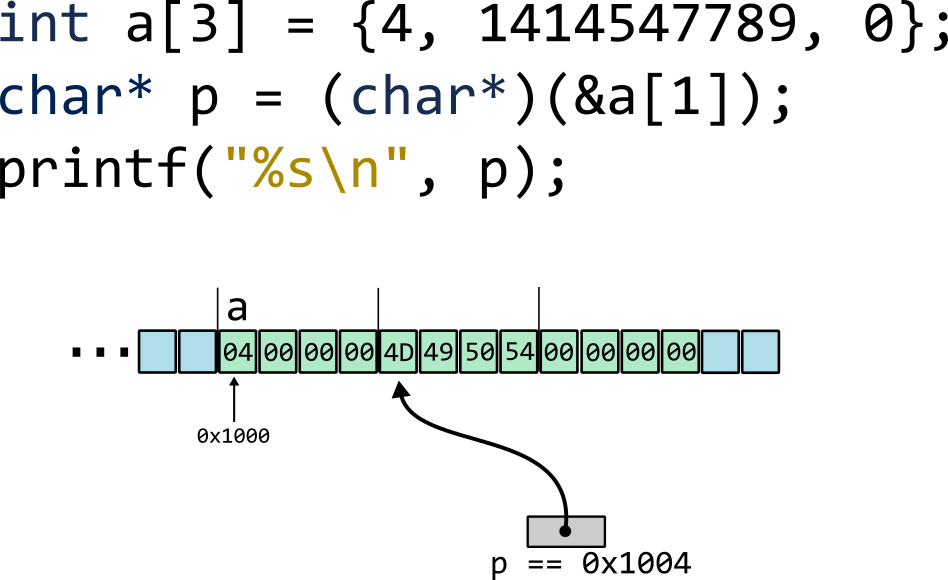
\includegraphics[width=0.86\linewidth]{../images/pointer_arithmetics/parithmetics_7_pointer_casting.png}
\end{center}
Что напечатает этот кусок кода?
\end{frame}

\begin{frame}[fragile]
\frametitle{Пример приведения указателей}
\begin{center}
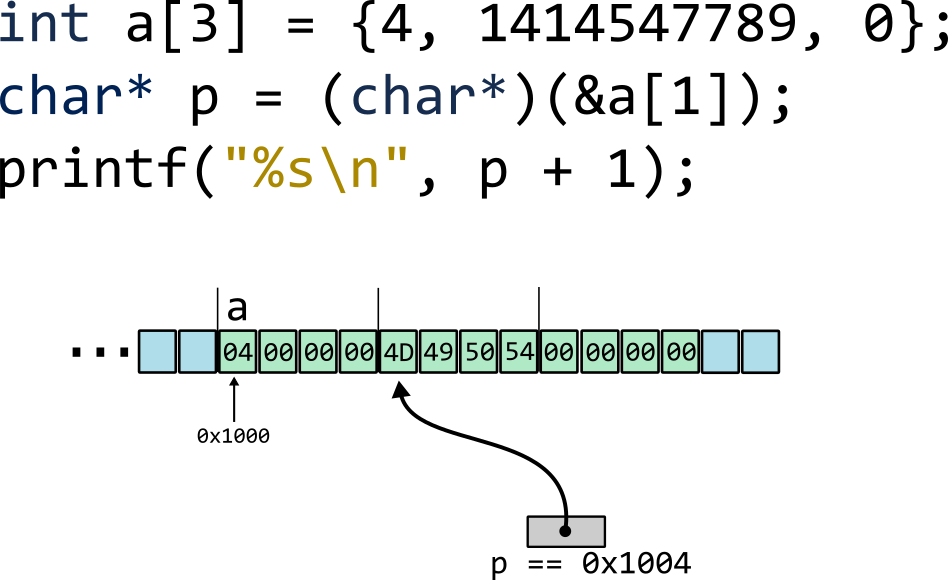
\includegraphics[width=0.86\linewidth]{../images/pointer_arithmetics/parithmetics_8_pointer_addition_and_casting.png}
\end{center}
Что напечатает этот кусок кода?
\end{frame}


\begin{frame}[fragile]
\frametitle{Указатель на \texttt{void}}
\begin{itemize}
\item Указатель, который на связан ни с каким типом
\begin{lstlisting}
void* p;
\end{lstlisting}
\item Его нельзя разыменовывать и применять другие операции
\item Но его можно привести к другому указателю:
\begin{lstlisting}
int a = 10;
void* p = (void*)&a;
*((int*)p) += 5;
\end{lstlisting}
\item Используется если нужно передать переменную, но её тип на момент написания кода неизвестен
\end{itemize}
\end{frame}

\section{Сегменты памяти}

\begin{frame}[fragile]
\frametitle{Сегменты памяти: общие моменты}
\begin{itemize}
\item Операционной системой предоставляется процессу адресное пространство
размером $2^{64}$ байт.
\item Это пространство делится на сегменты
\item При попытке чтения/записи ячейки памяти недоступного для записи сегмента
возникает ошибка \texttt{SegmentationFault}
\item Для каждого процесса область памяти независима от других процессов. 
Т.е. нельзя случайно повредить память другого процесса.
\end{itemize}
\end{frame}

\begin{frame}[fragile]
\frametitle{Сегменты памяти}
\begin{center}
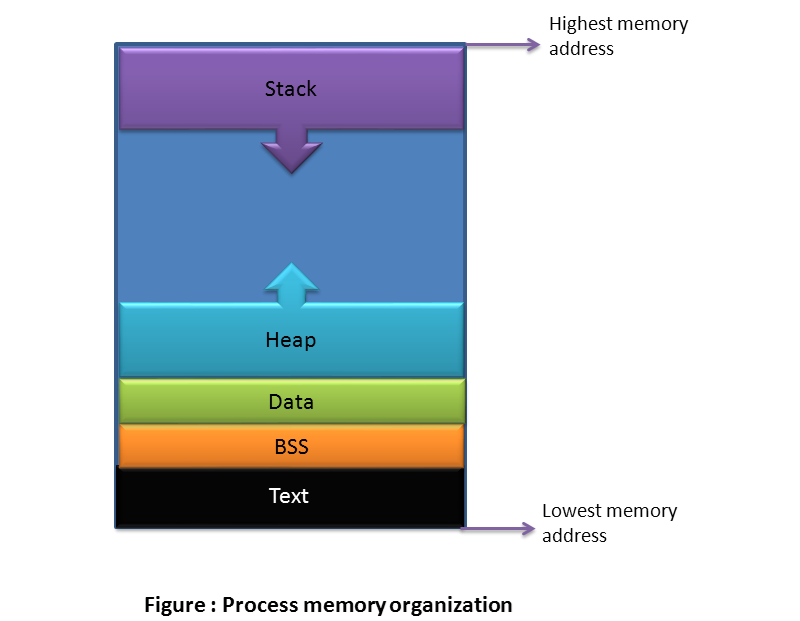
\includegraphics[width=0.86\linewidth]{../images/process_memory_organization.png}
\end{center}
\end{frame}


\begin{frame}[fragile]
\frametitle{Сегмент памяти Стек (Stack)}
\begin{itemize}
\item В этом сегменте создаются все переменные и статические массивы
\begin{lstlisting}
int a;
float b[10];
\end{lstlisting}
\item Имеет небольшой размер, определяемый операционной системой (обычно не более 10 мегабайт)
\item Быстрее выделяется память, чем в Куче
\item Память выделяется в начале выполнения функции(под все локальные переменные) и освобождается
при завершении функции
\end{itemize}
\end{frame}


\begin{frame}[fragile]
\frametitle{Сегмент памяти Куча (Heap)}
\begin{itemize}
\item В этом сегменте выделяется динамическая память
\begin{lstlisting}
int* p = malloc(100);  // Выделим 100 байт
\end{lstlisting}
\item Имеет размер, ограниченный только свободной оперативной памятью
\item Медленней выделяется память, чем в Стеке
\item Память выделяется с помощью функции \texttt{malloc} или аналогов и освобождается с помощью функции
\texttt{free} в любом месте программы.
\end{itemize}
\end{frame}

\end{document}
